% Standalone gallery of every figure used in main.tex
% Compile: cd paper && pdflatex figures_gallery.tex
\documentclass[11pt]{article}
\usepackage[margin=0.75in]{geometry}
\usepackage{graphicx}
\usepackage{booktabs}
\usepackage{caption}
\usepackage{subcaption}
\usepackage[hidelinks]{hyperref}

\graphicspath{{figures/}}

\title{LEMC Paper --- Figure Gallery}
\author{All images referenced in \texttt{main.tex}}
\date{}

\begin{document}
\maketitle

This document lists the \textbf{13 image files} used in the conference paper.
Source paper: \texttt{paper/main.tex}. Images live in \texttt{paper/figures/}.

\section{Full-width figures}

\begin{figure}[ht]
  \centering
  
\includegraphics[width=\linewidth,keepaspectratio]{fig2_architecture.png}
  \caption{\texttt{fig2\_architecture.png} --- Fixed ORB-affine pipeline (Fig.~2 in paper).}
\end{figure}

\begin{figure}[ht]
  \centering
  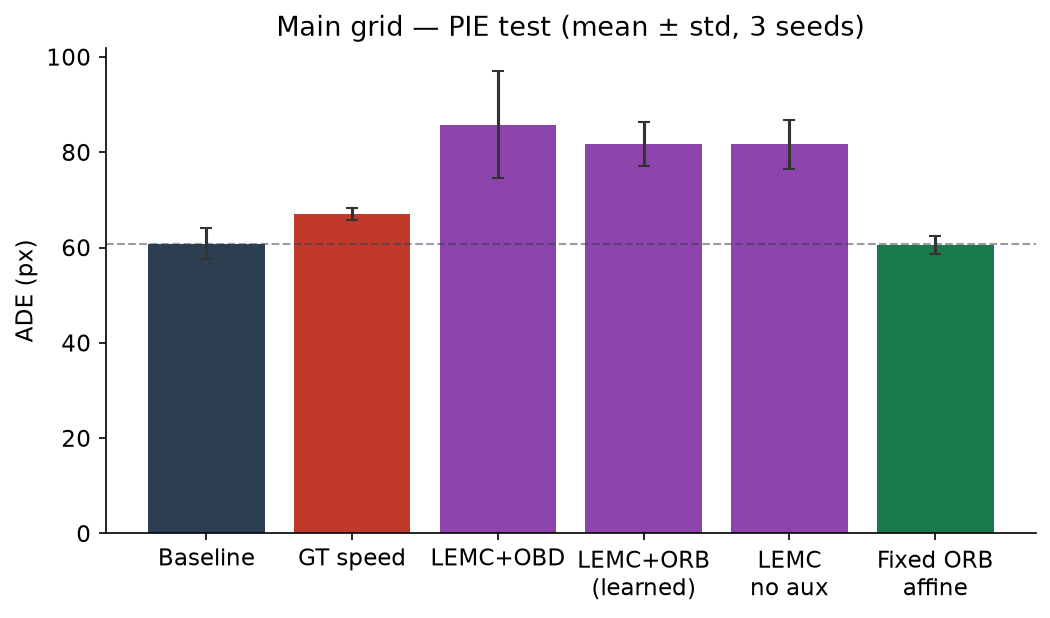
\includegraphics[width=\linewidth,keepaspectratio]{fig_main_grid_ade.png}
  \caption{\texttt{fig\_main\_grid\_ade.png} --- PIE ADE grid (Fig.~3).}
\end{figure}

\section{Two-panel diagnostic figures}

\begin{figure}[ht]
  \centering
  \begin{subfigure}[t]{0.48\linewidth}
    \centering
    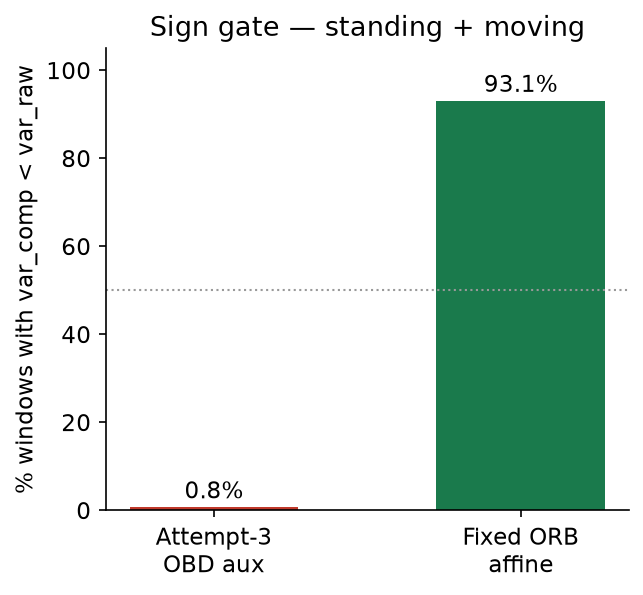
\includegraphics[width=\linewidth,keepaspectratio]{fig_sign_gate.png}
    \caption{Sign gate}
  \end{subfigure}\hfill
  \begin{subfigure}[t]{0.48\linewidth}
    \centering
    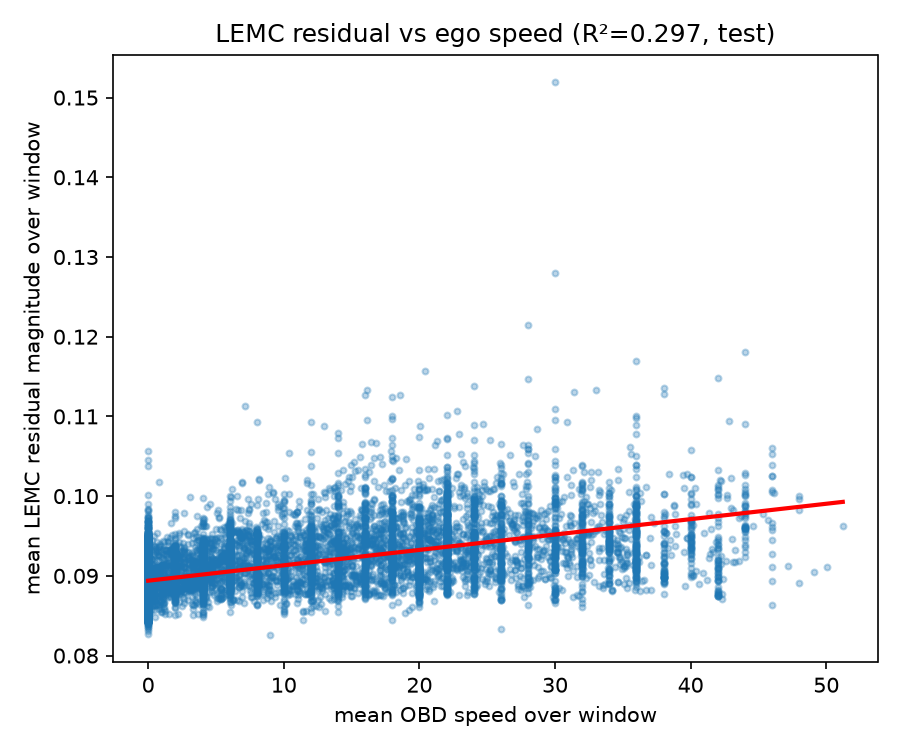
\includegraphics[width=\linewidth,keepaspectratio]{lemc_obd_scatter_pie_lemc_augmented_auxobd_seed0_test.png}
    \caption{LEMC vs.\ OBD scatter}
  \end{subfigure}
  \caption{\texttt{fig\_sign\_gate.png}, \texttt{lemc\_obd\_scatter\_...png} --- Variance gate diagnostics (Fig.~4).}
\end{figure}

\begin{figure}[ht]
  \centering
  \begin{subfigure}[t]{0.48\linewidth}
    \centering
    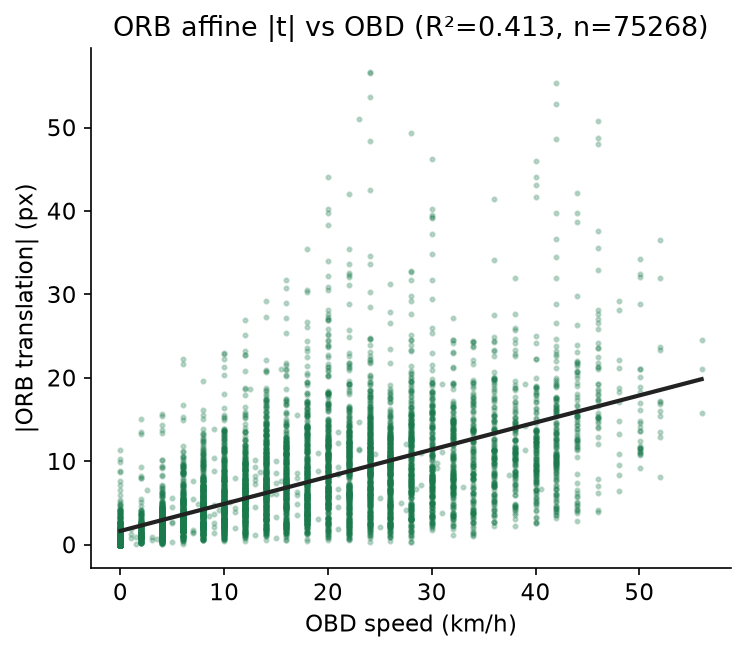
\includegraphics[width=\linewidth,keepaspectratio]{fig4_orb_obd_scatter.png}
    \caption{ORB vs.\ OBD}
  \end{subfigure}\hfill
  \begin{subfigure}[t]{0.48\linewidth}
    \centering
    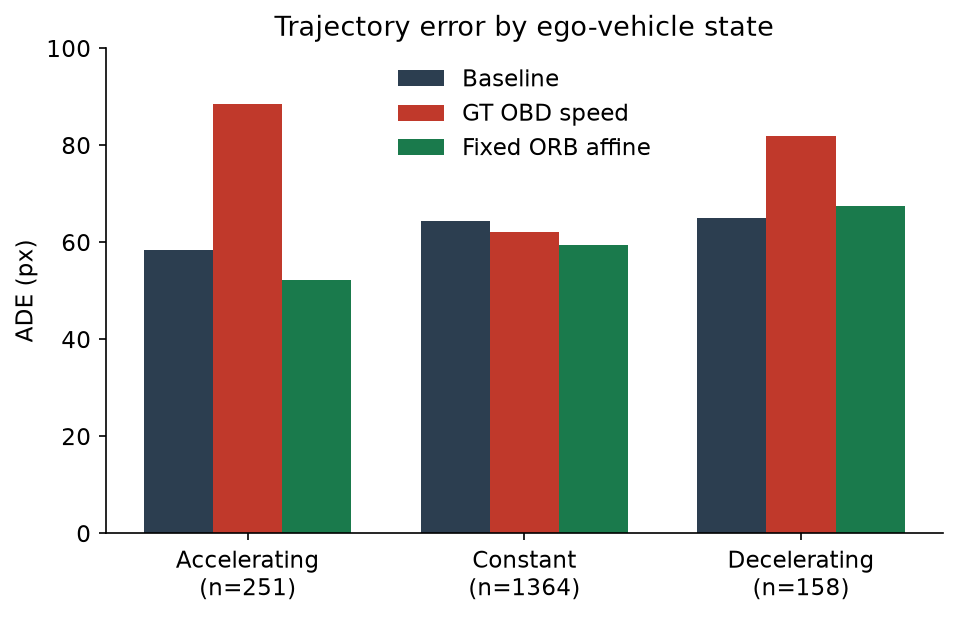
\includegraphics[width=\linewidth,keepaspectratio]{fig5_stratified_ade.png}
    \caption{Stratified ADE}
  \end{subfigure}
  \caption{\texttt{fig4\_orb\_obd\_scatter.png}, \texttt{fig5\_stratified\_ade.png} --- ORB validation (Fig.~5).}
\end{figure}

\section{JAAD cross-dataset}

\begin{figure}[ht]
  \centering
  \begin{subfigure}[t]{0.30\linewidth}
    \centering
    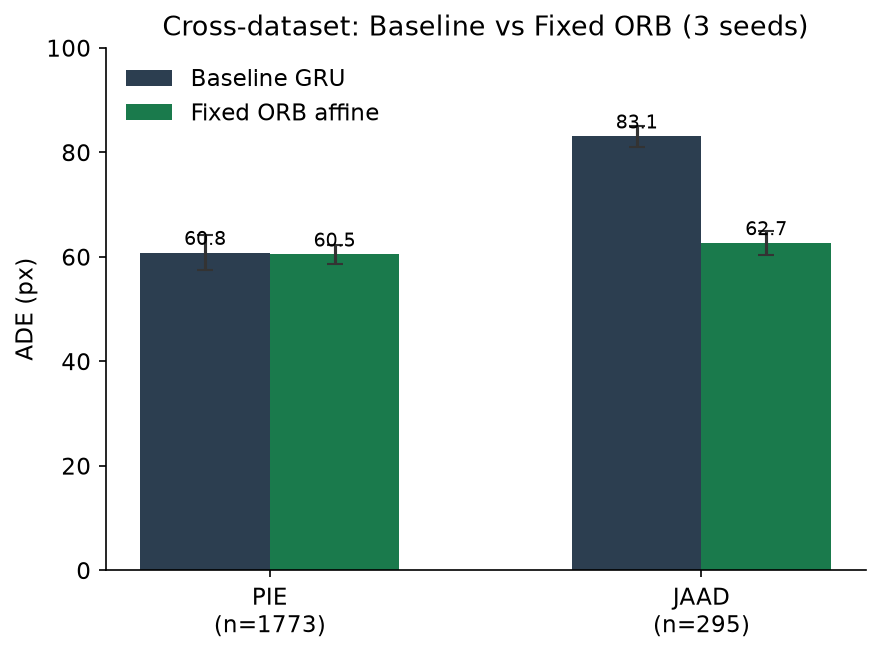
\includegraphics[width=\linewidth,keepaspectratio]{cross_dataset_ade.png}
    \caption{Cross-dataset ADE}
  \end{subfigure}\hfill
  \begin{subfigure}[t]{0.34\linewidth}
    \centering
    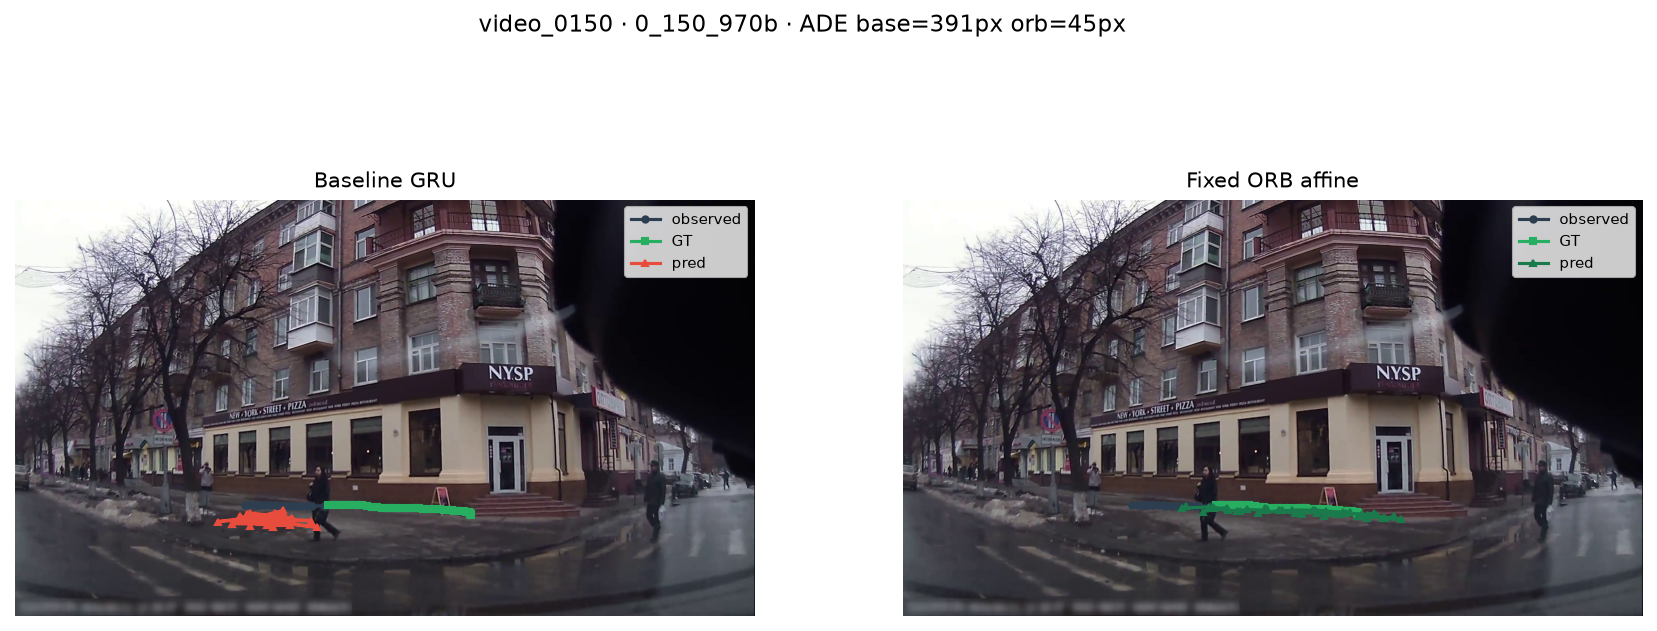
\includegraphics[width=\linewidth,keepaspectratio]{jaad_compare_0.png}
    \caption{JAAD video 0150}
  \end{subfigure}\hfill
  \begin{subfigure}[t]{0.34\linewidth}
    \centering
    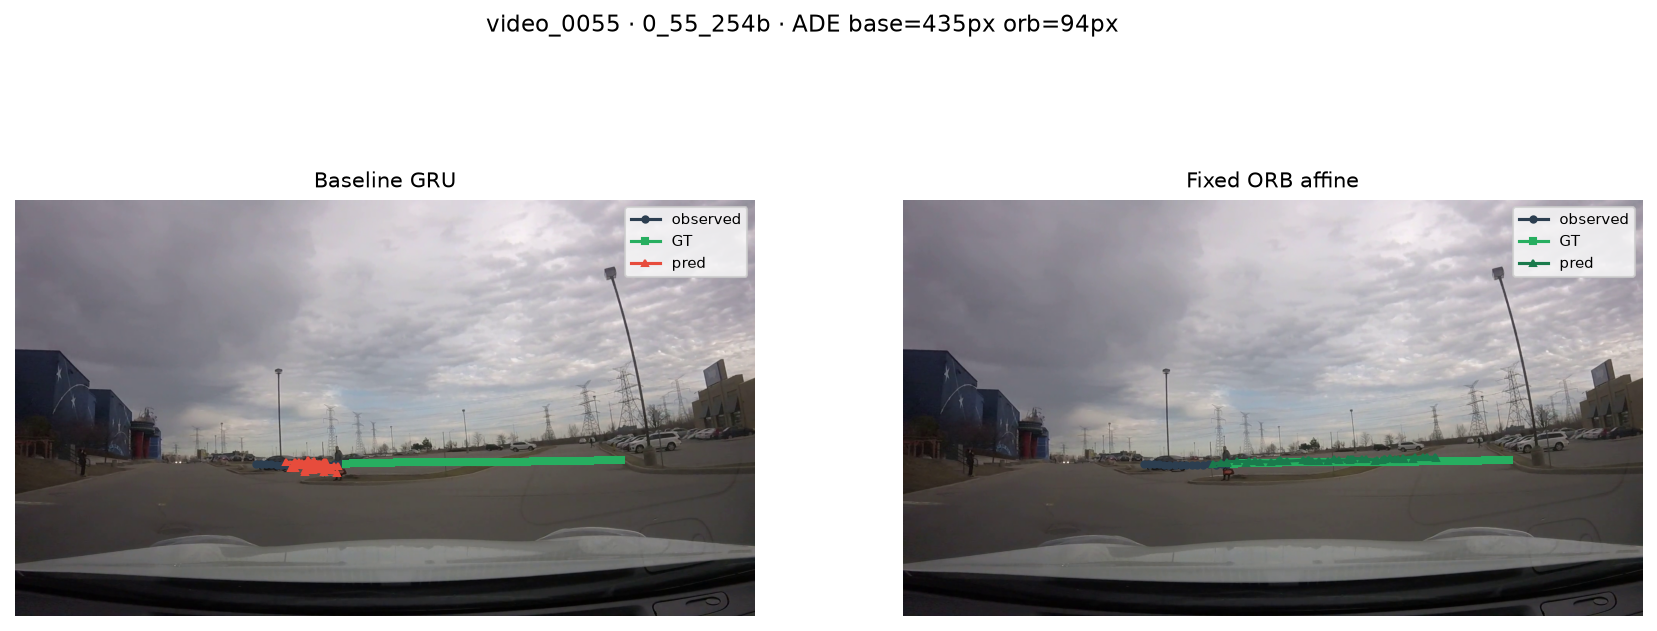
\includegraphics[width=\linewidth,keepaspectratio]{jaad_compare_1.png}
    \caption{JAAD video 0055}
  \end{subfigure}
  \caption{\texttt{cross\_dataset\_ade.png}, \texttt{jaad\_compare\_0.png}, \texttt{jaad\_compare\_1.png} --- JAAD results (Fig.~6).}
\end{figure}

\section{Qualitative summary (four-panel)}

\begin{figure}[ht]
  \centering
  \begin{subfigure}[t]{0.24\linewidth}
    \centering
    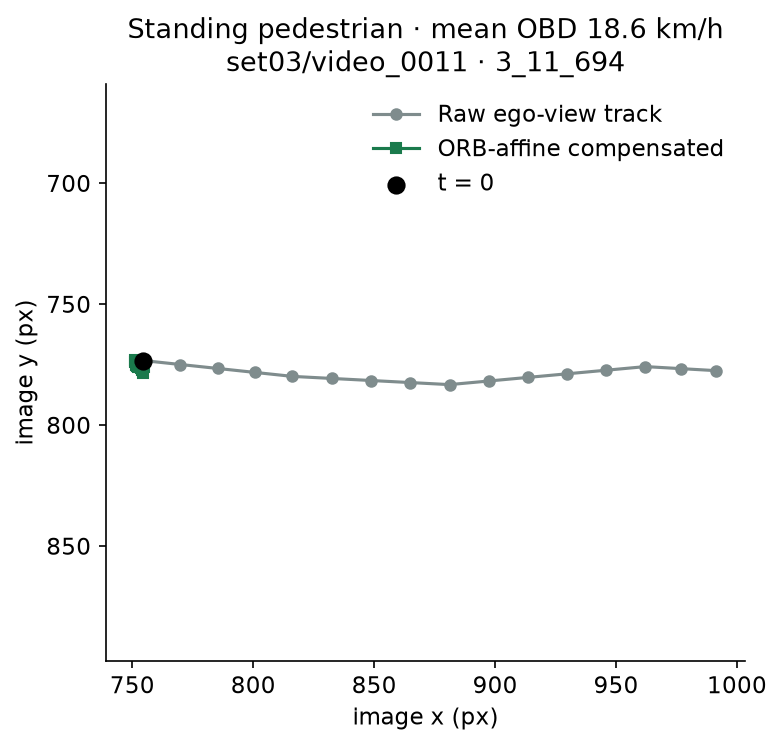
\includegraphics[width=\linewidth,keepaspectratio]{fig1_teaser.png}
    \caption{Standing pedestrian}
  \end{subfigure}\hfill
  \begin{subfigure}[t]{0.24\linewidth}
    \centering
    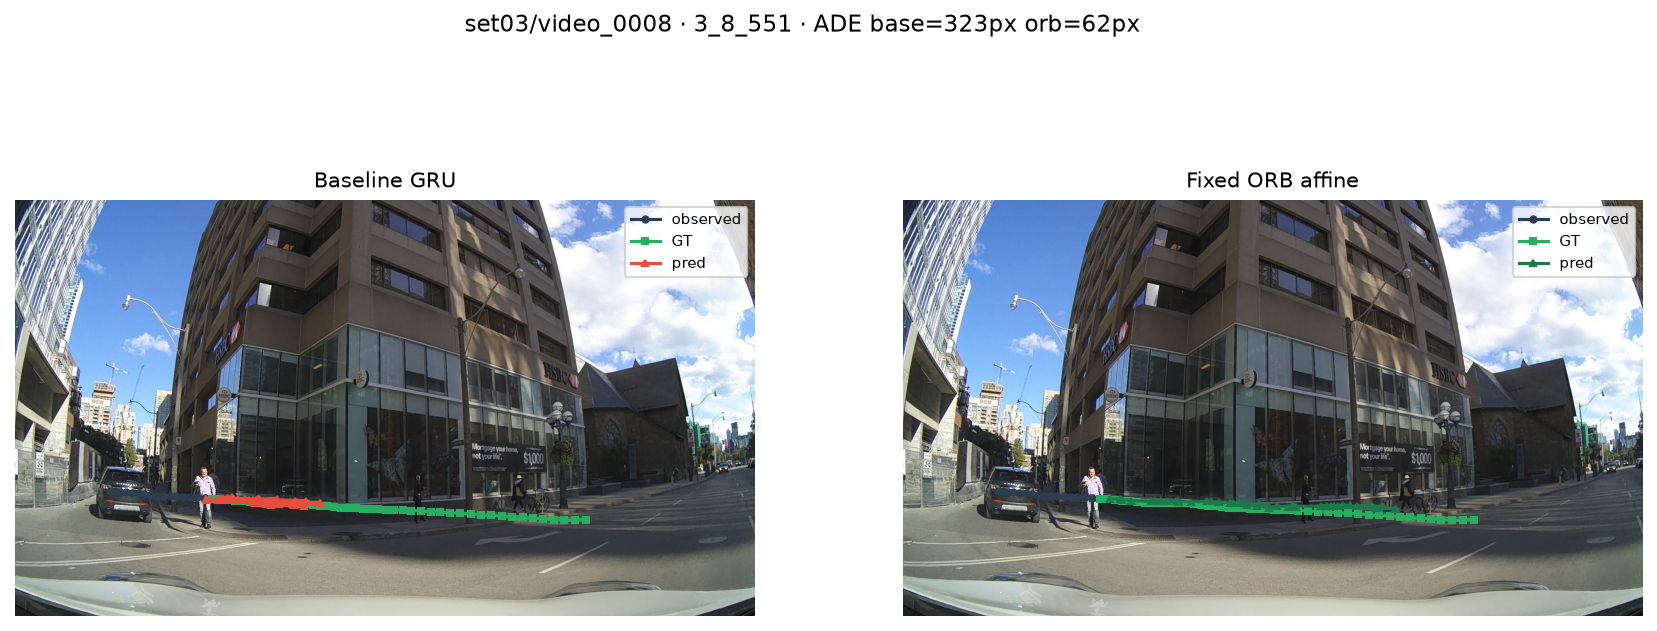
\includegraphics[width=\linewidth,keepaspectratio]{pie_compare_0.png}
    \caption{PIE overlay}
  \end{subfigure}\hfill
  \begin{subfigure}[t]{0.24\linewidth}
    \centering
    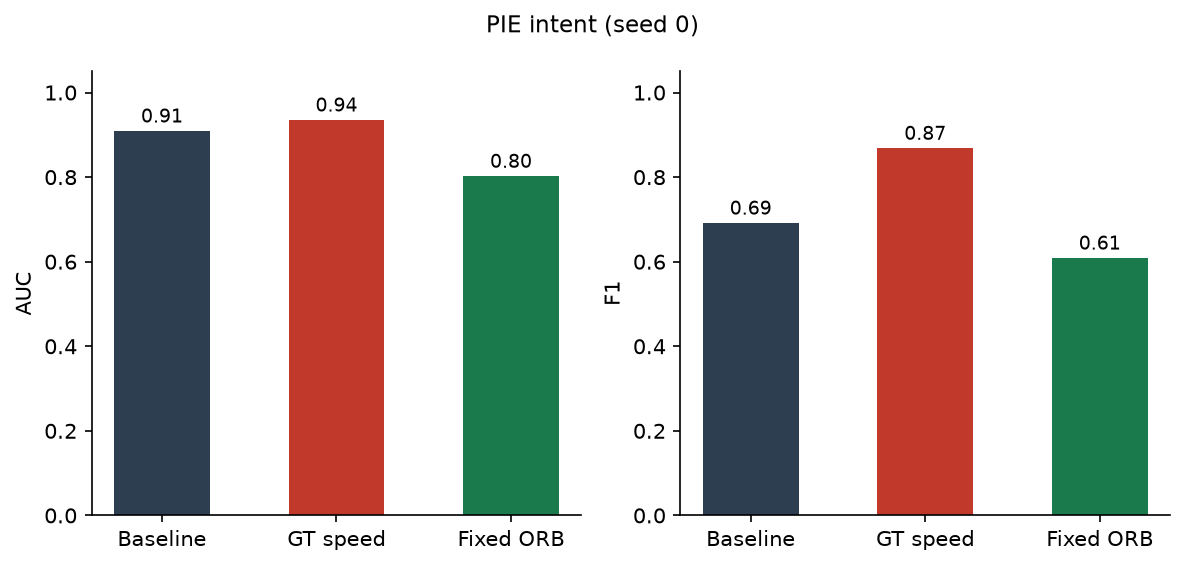
\includegraphics[width=\linewidth,keepaspectratio]{pie_intent_auc_f1.png}
    \caption{Intent AUC/F1}
  \end{subfigure}\hfill
  \begin{subfigure}[t]{0.24\linewidth}
    \centering
    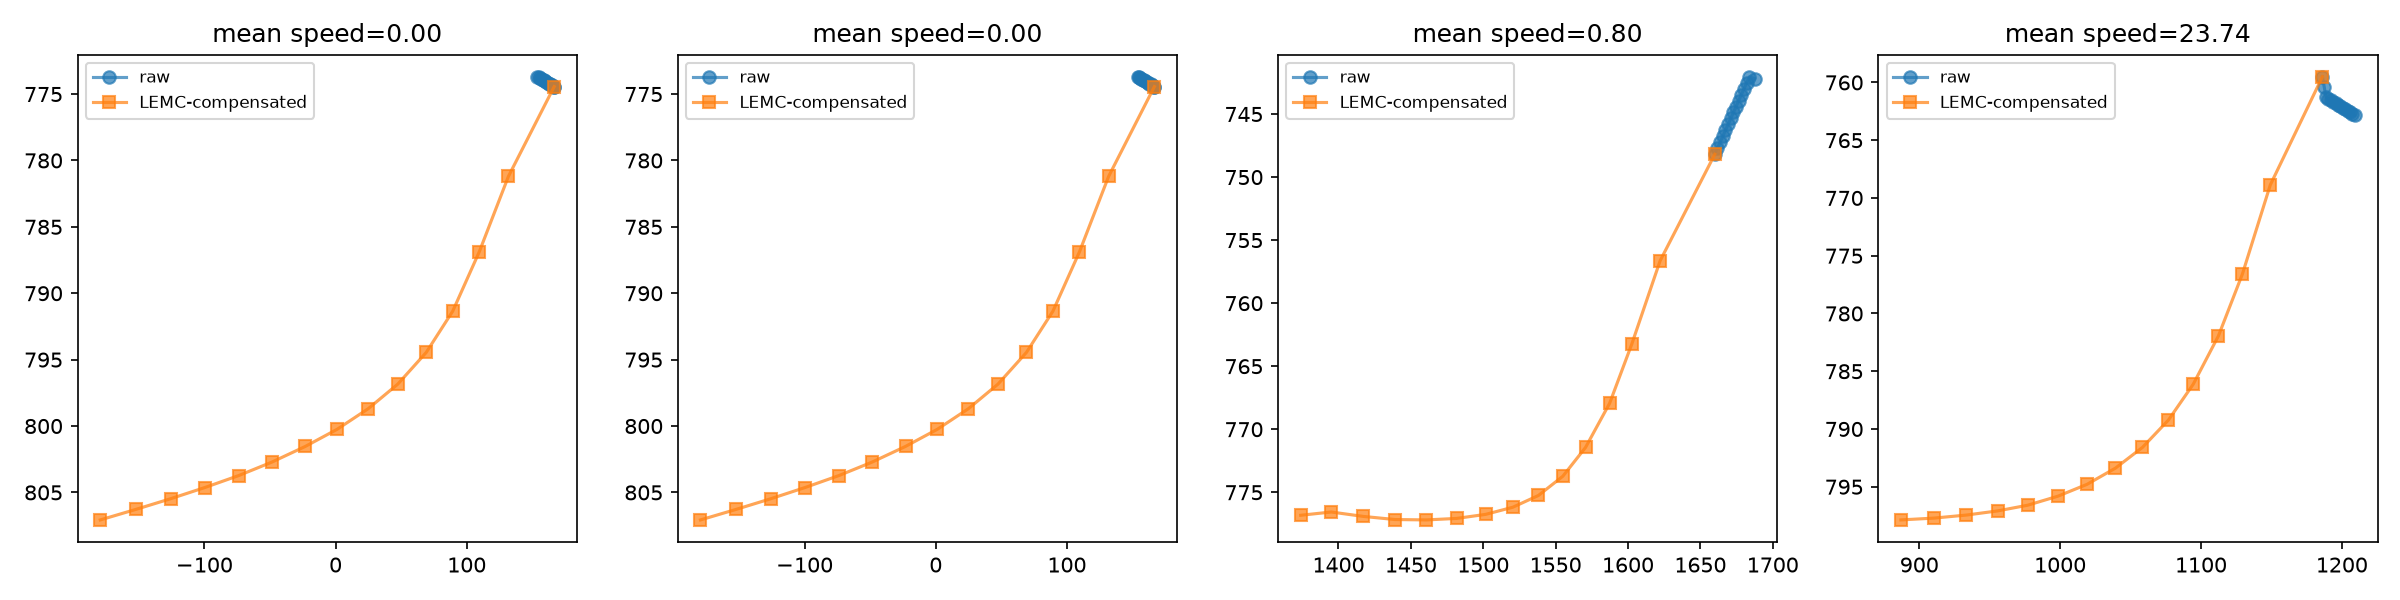
\includegraphics[width=\linewidth,keepaspectratio]{lemc_qualitative_pie_lemc_augmented_auxobd_seed0_test.png}
    \caption{LEMC failure}
  \end{subfigure}
  \caption{\texttt{fig1\_teaser.png}, \texttt{pie\_compare\_0.png}, \texttt{pie\_intent\_auc\_f1.png}, \texttt{lemc\_qualitative\_...png} --- Qualitative summary (Fig.~7).}
\end{figure}

\section{Image manifest}

\begin{table}[ht]
  \centering
  \footnotesize
  \begin{tabular}{@{}lll@{}}
    \toprule
    File & Paper figure & Section \\
    \midrule
    \texttt{fig2\_architecture.png} & Fig.~2 & Method \\
    \texttt{fig\_main\_grid\_ade.png} & Fig.~3 & PIE main grid \\
    \texttt{fig\_sign\_gate.png} & Fig.~4a & Variance gate \\
    \texttt{lemc\_obd\_scatter\_pie\_lemc\_augmented\_auxobd\_seed0\_test.png} & Fig.~4b & Variance gate \\
    \texttt{fig4\_orb\_obd\_scatter.png} & Fig.~5a & ORB validation \\
    \texttt{fig5\_stratified\_ade.png} & Fig.~5b & Stratified PIE \\
    \texttt{cross\_dataset\_ade.png} & Fig.~6a & JAAD \\
    \texttt{jaad\_compare\_0.png} & Fig.~6b & JAAD \\
    \texttt{jaad\_compare\_1.png} & Fig.~6c & JAAD \\
    \texttt{fig1\_teaser.png} & Fig.~7a & Qualitative \\
    \texttt{pie\_compare\_0.png} & Fig.~7b & Qualitative \\
    \texttt{pie\_intent\_auc\_f1.png} & Fig.~7c & Qualitative \\
    \texttt{lemc\_qualitative\_pie\_lemc\_augmented\_auxobd\_seed0\_test.png} & Fig.~7d & Qualitative \\
    \bottomrule
  \end{tabular}
  \caption{All PNG files included by \texttt{main.tex}.}
\end{table}

\noindent\textbf{Not used in paper:} \texttt{fig3\_qualitative.png} (superseded by the four-panel qualitative figure).

\end{document}
